\chapter{Como Funcionam as Defesas na Coppe}
\label{app:coppedef}

Neste apêndica se faz um breve resumo de como as coisas acontecem no Programa de Engenharia de Sistemas e Computação da Coppe.

\section{Seminário de Qualificação de Mestrado}

Na Coppe, existe o Seminário de Qualificação de Mestrado, com prazo improrrogável de 2 anos, onde a aprovação é feita só pelo professor. É comum, porém, que exista uma banca que apoia o orientador.

A minha prática é exigir um documento na forma de artigo que faça uma revisão do tema da dissertação e proponha e justifique um projeto de dissertação, com objetivos e cronograma. Para a defesa, o aluno deve fazer uma apresentação.

\section{O Exame de Qualificação de Doutorado}

Na Coppe, o exame de qualificação tem um prazo máximo de três anos. Como o prazo da bolsa é de quatro anos, e o da defesa é de cinco anos, é comum que o exame seja feito em um tempo que consideramos de cedo. Para mim, entre dois anos e dois anos e meio o aluno já devia ser capaz de fazê-lo.


\section{A Defesa de Mestrado e Doutorado}

A defesa de dissertação de mestrado é feita por uma banca com no mínimo 3 pessoas, com pelo menos um membro externo e outro interno. 
Já a defesa de tese de doutorado exige uma banca de cinco pessoas, com dois membros externos obrigatórios, sendo que um deles, pelo menos, deve ser externo à UFRJ.

Uma defesa de tese é uma \textbf{apresentação formal} da mesma, na forma de um seminário, pelo candidato, a uma banca de doutores.

Esses doutores são propostos pelo orientador, normalmente, mas não necessariamente, em acordo com o orientado, a um órgão colegiado\footnote{Na Coppe, a CPGP}, que aprova, ou não, a escolha. O orientador escolhe os membros da banca conforme o tema, a experiência e o reconhecimento dos professores convidados, e questões de logística, como disponibilidade nas datas previstas, disponibilidade de verba, etc.

Dependendo do programa, a defesa pode ser realizada na forma presencial, remota ou híbrida. Após a pandemia, e também por dificuldades de verba para viagem de professores, as formas remota e híbrida passaram a ser muito mais aceitas entre os programas.

O candidato deve entregar a sua tese  à banca e ao registro 15 dias antes.


\subsection{Como as Coisas Acontecem na Defesa}

Nesta seção se faz uma narrativa do processo específico da defesa.

\begin{enumerate}
    \item O presidente da banca anuncia o início da defesa, indicando o candidato, o nome da tese, o orientador (normalmente o próprio presidente da banca), a banca (agradecendo a presença) e passa a palavra ao candidato;
    \item O candidato faz a apresentação, na forma de uma palestra de 40 a 50 minutos, onde não pode ser interrompido;
    \item O presidente inicia o processo de comentários e arguição, passando a palavra ao primeiro membro a falar, normalmente ordenando do membro mais externo para o mais interno, sendo os orientadores os últimos a falar;
    \item em sua vez de falar, os membros da banca podem, ou não, fazer perguntas para ser respondidas imediatamente, ou no final de sua fala, ao candidato;
    \item após os membros da banca comentarem a dissertação ou questionarem os candidatos sobre a mesma, a palavra é passada a plateia, que pode ou não se manifestar (normalmente não se manifesta);
    \item o candidato e a plateia se retiram da sala para a banca deliberar (ou banca se retira, principalmente em defesas virtuais);
    \item a banca convoca o candidato e plateia para ler o resultado;
    \item o resultado é lido;
    \item a ata é assinada e se encerra a defesa.
\end{enumerate}


\section{Questões Administrativas}

Você tem que defender antes do fim do seu prazo. 

Você deve estar ciente de todas as regras da defesa e, também, de suas obrigações antes e depois da defesa, que estão disponíveis nos sites do PESC, da Coppe e do Registro da Coppe.

Aqui são listadas apenas algumas informações mais constantes, porém pouca da burocracia e dos documentos necessários.

\section{Acompanhamento de Processos}
A maioria dos pedidos oficiais é feita por meio de um processo pelo sistema SEI, da UFRJ, que pode ser acompanhado pelo aluno por meio do link \url{https://sei.ufrj.br/pesquisa}. Para isso, busque por PROCESSOS (só marque essa caixa) com seu nome completo no campo ``Interessado'', e após descobrir o processo importante, anote o número dele. Veja um exemplo de tela na \autoref{fig:sei}.

\begin{figure}[hbt]
    \centering
    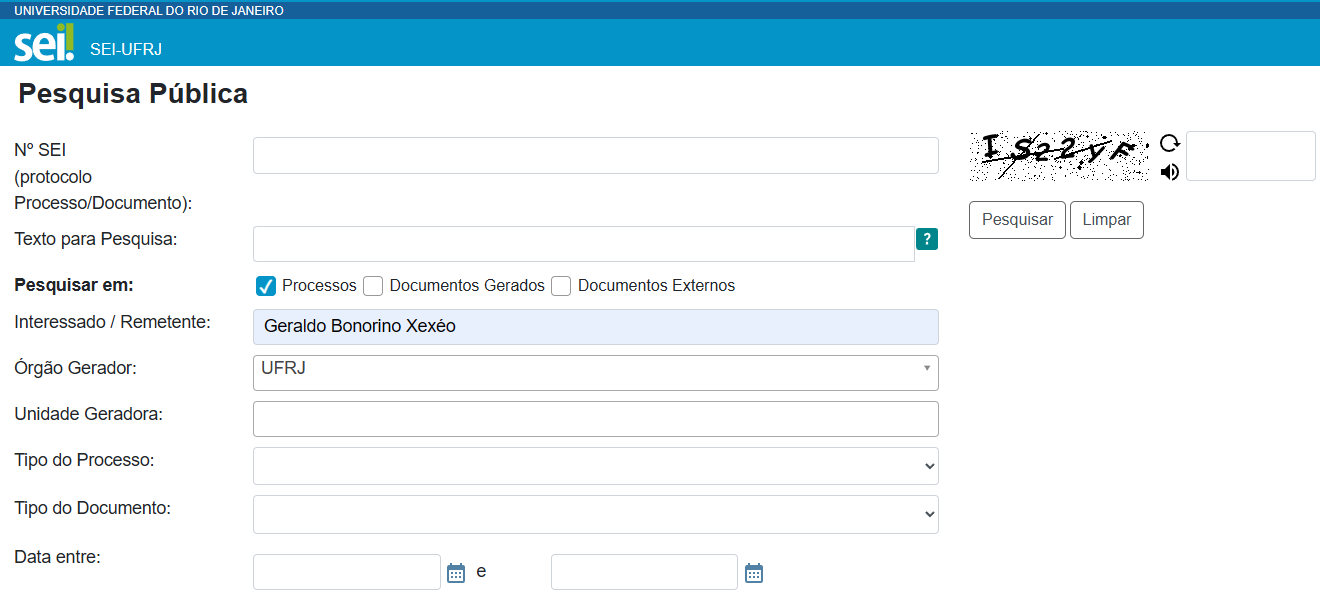
\includegraphics[width=\linewidth]{Images/SEIPesquisa.png}
    \caption{Tela do SEI Pesquisa}
    \label{fig:sei}
\end{figure}

Os processos importantes na defesa são:
\begin{itemize}
    \item Pós-Graduação: Homologação de Candidatura - Qualificação (Stricto Sensu), que tem que estar aprovado para pedir banca.
    \item Pós-Graduação: Aprovação de Banca Examinadora e Homologação de Defesa (Stricto Sensu), que é usado desde o pedido de banca até a entrega do diploma.

\end{itemize}

Outros processos que podem ocorrer:
\begin{itemize}
    \item Pós-Graduação: Mudança de Orientação (Substituição, Inclusão ou Exclusão), se houve mudança na orientação original, como a inclusão de membro externo a Coppe.
    \item Pós-Graduação: Aproveitamento de Disciplina (Stricto Sensu), se foram feitas cadeiras fora da Coppe. 
        \item Pós-Graduação: Prorrogação de Prazo para a Defesa de Dissertação/Tese (Stricto Sensu), se houve prorrogação
\end{itemize}

Os processos são aprovados no PESC, possivelmente pelo Coordenador Acadêmico ou pelo Colegiado em alguns casos, e depois na CPGP. Para saber que um processo foi aprovado é necessário buscar o parecer que indica a aprovação pela CPGP. 

Tirando o período de recesso no fim de ano, a CPGP normalmente se reúne as terças-feiras de manhã e, na quase totalidade dos casos, aprova o parecer do relator, que pode ser favorável, desfavorável, ou fazer exigências. Essas decisões estão listadas como ``Parecer''. Por isso, quando há o parecer favorável do relator, se tem quase certeza que na próxima terça-feira a CPGP aprovará o parecer e o pedido. Se há um parecer desfavorável, ainda há tempo de fazer as correções necessárias.

O professor da Coppe tem acesso a uma interface um pouco mais rica e também experiência em interpretar o que está acontecendo, por exemplo, por que um pedido está parado.


\section{Antes da Sua Defesa}

Uma lista de ações obrigatórias para a defesa acontece, e cujas regras variam ao longo do tempo.

\begin{itemize}
    \item Seu orientador deve pedir a banca com até 45 dias de antecedência da data prevista de defesa, que deve ser antes do fim de seu prazo para defesa. 
    \item Você deve depositar a dissertação no registro, provavelmente por meio de uma cópia em PDF salva no software \verb|ctrl-pesc|, \textbf{até 15 dias antes da defesa real (e não da data prevista no pedido)}
    \item Você deve enviar cópias a banca, também até 15 dias antes da defesa, há um documento que informa esse envio ao registro.
    \item A data e o horário finais da defesa tem que ser acordados entre banca e candidato.
    \item Deve ser marcada a sala ou criada a sala virtual.
    \item Deve ser feito um anúncio público e formal da defesa, que será registrado no site do PESC.
    \item O orientador deve pedir a ata para o registro, uns dois ou três dias antes, mas para isso o aluno tem que ter enviado, além da cópia da dissertação em PDF, alguns documentos exigidos pelo registro e que precisam da assinatura do aluno e do orientador. Há um email padrão para isso.
    \item O orientador deve receber a ata digital ou passar no registro para pedir a ata de papel (para isso é necessário avisar antes que vai querer uma ata de papel)
\end{itemize}


\section{Escolha e convite da banca}

Todos os membros da banca devem passar pelo crivo da Coppe, que exige o doutorado e em torno de 1 artigo em revista acadêmica indexada por ano, nos últimos quatro anos, em média. Além disso, é considerada a ligação do membro da banca com o orientador, e a experiência geral do mesmo. Essa análise é feita por meio do currículo Lattes. Isso significa que se um membro proposto não é doutor e não tem pelo menos 3 artigos em revistas indexadas\footnote{Uma revista acadêmica indexada deve constar de índices reconhecidos, principalmente o JCR Web of Science}

Documento oficial que deve ser feito pelo menos 45 dias antes da defesa. A data marcada no pedido, porém, não é obrigatório. Aprovada a banca, pode ser defendida antes (até agora), ou depois. O procedimento de pedido de banca é iniciado pelo professor, mas depende de documentos do aluno. O pedido é processado pela secretaria acadêmica.


\section{Reserva de sala}

A sala é reservada na secretaria, com uma pasta específica para isso. Em caso de sala virtual, deve ser divulgado o link e ele deve ser público e aberto para o público. 

\section{Depois de Sua Defesa}

Depois de sua defesa, a maior parte das obrigações é sua. O orientador apenas vai enviar a ata para o registro. Você deve fazer todo o resto da documentação no prazo hábil. No caso de reprovação, pouco ou nada há a ser feito.

No caso de aprovação por unanimidade, esse prazo é de 30 dias. Durante esse tempo, o orientador deve conversar com você sobre as modificações necessárias a partir dos comentários e perguntas da banca.

No caso de aprovações com exigências, o candidato ainda não foi aprovado. Ao fazer as modificações pedidas, o candidato deve prestar contas e interagir com o orientador e o fiscal.

Nesses dois últimos casos, muito mais frequentes, há vários passos descritos na documentação. Esses passos permitirão que seu diploma seja pedido e seu registro marque que você recebeu o grau de mestre.

Dois passos são importantes, o depósito da versão final da dissertação no registro, para o qual há um prazo fixo e que não pode ser prorrogado, e o depósito da dissertação no PESC, essencial para o prosseguimento do processo de requisição do diploma.

Além disso, é gentil e praticamente obrigatório enviar a versão final da dissertação para a banca, em PDF.


\needspace{5\baselineskip}
\section{Prazo}

O prazo para defesa de dissertação de mestrado é de 3 anos. Ele é contado sempre a partir da data de matrícula no SIGA, que está tanto no Boletim quanto no Histórico Escolar do aluno. Recentemente, a contagem do prazo passou a ser interrompida quando o aluno tranca matrícula, e ainda há outras condições possíveis de interrupção do prazo, como licença médica para maternidade. Esse prazo pode ser prorrogado em até 6 meses, mediante justificativa válida e concordância do orientador.

O pedido de prorrogação, se feito, deve ser feito \textbf{antes do prazo acabar.} O aluno não deve contar com a aprovação\footnote{Não concordarei com pedidos que não sejam embasados em causa grave, o que exclui a falta de tempo por estar trabalhando, e outras condições que poderiam ter sido controladas pelo aluno}.


Como calcular a sua data provável de defesa e quando fazer os pedidos:
\begin{outline}
    \1 Calcule, ou faça uma previsão, do seu último dia de defesa.
    \2 A sua data máxima de defesa é 3 anos depois do seu dia de matrícula no SIGA.
    \2 É fortemente recomendado que você defenda em 2 anos, principalmente se for bolsista.
    \1 Considere que é muito difícil fazer defesas entre 15 de dezembro e janeiro até o início de março.
    \1 Considere uma margem de 15 a 30 dias para possibilitar a marcação da banca em um dia em que todos os professores estarão disponíveis.
    \1 Considere 45 dias antes para pedir a banca.
    \2 Considere que a CPGP, o órgão que aprova a banca, entra em recesso de meados de dezembro a fim de janeiro.
    \1 Considere 15 dias antes para o orientador poder escolher e convidar a banca.
\end{outline}

Por exemplo, se sua matrícula é 1\textsuperscript{o} de março de 2025, com o prazo de 3 anos, você tem que defender até 1\textsuperscript{o} de março de 2028. Porém não vai ser prático fazer isso. Considere então que sua defesa poderá ser entre 15 de novembro de 2027 e 15 de dezembro de 2027. Subtraia 45 dias, chegando a 1\textsuperscript{o} de outubro de 2027, logo deve, em torno de 15 de setembro de 2027, solicitar ao orientador escolher, convidar e pedir a banca.

Se você percebeu, há uma espécie de ``redução do prazo'' na prática. Você tinha 3 anos, mas será muito difícil defender em 3 anos nesse caso. O prazo também não desconta feriados, como o carnaval, etc.

Claro que o plano é que você defenda em torno de 2 anos, assim, você pode pensar que vai defender entre 15 de março e 15 de abril de 2027, o que passa o momento de discutir a banca com o orientador para outubro de 2026.



\section{Os Resultados}

Existem três resultados possíveis:
\begin{itemize}
    \item \textbf{Aprovação da dissertação por unanimidade}: significa que você foi aprovado sem modificações de relevância. A banca, e a instituição, ainda esperam que algumas modificações sugeridas sejam feitas, e o aluno tem 30 dias para depositar a versão final no registro e no PESC. O orientador pode ou não auxiliar nas modificações, dependendo da importância delas.
    \item \textbf{Aprovação  somente  após  satisfazer  as  exigências que constam 	 na  folha  de   modificações  no  prazo   fixado  pela  banca    ( não superior  a   noventa   dias)}: nesse caso, que é comum, será criada uma ata adicional com uma lista de mudanças, e haverá um ou dois indicados para verificar as modificações foram feitas. Normalmente isso significa que a banca reconhece que foi feito um trabalho que quase atingiu o nível necessário do mestrado, mas que precisa de esforços adicionais, ou que precisa de grandes correções de texto.
    \item \textbf{Reprovação da dissertação}: uma ocorrência rara, mas possível, e provavelmente indicada anteriormente pelo orientador sobre sua possibilidade. Indica que o aluno não atingiu o mínimo desejável para o bter o título de mestrado. Já vi algumas reprovações, sendo que os motivos incluíram plágio, experiências não realizadas, e baixa qualidade total do trabalho que tinha sido avisada pelo orientador.
\end{itemize}


% \section{Sobras}


% A banca deve cumprir requisitos, atualmente segundo o regulamento que pode ser obtido  no Espaço do Aluno no site da Coppe (Ver em URLs).
% \footnote{Endereço direto na data de edição deste texto: \url{https://coppe.ufrj.br/wp-content/uploads/2024/06/diretrizesbancas.pdf}}. Esses requisitos fazem exigências quanto à experiência comprovada e avaliação do professor segundo as mesmas regras da Coppe.

% O prazo é de 3 anos para o aluno de mestrado, contados a partir do dia de matrícula que está em seu Histórico Escolar e Boletim.

% Em caso de forma híbrida ou presencial, o candidato deve entregar um documento de concordância. 
% }
